\chapter{Теоретические основы динамической симуляции огня}

В общем случае задача симуляции огня может быть разбита на три
непересекающихся подзадачи~\cite{Perry94synthesizingflames}:
\begin{itemize}
	\item моделирование;
	\item анимация;
	\item визуализация.
\end{itemize}

В первую очередь необходимо выбрать подходящую внутреннюю структуру, или модель,
для симуляции. Далее, требуется выбрать способ анимации --- метод, с помощью
которого будет происходить взаимодействие с моделью. Техника анимации служит для
того, чтобы оживить модель, привести ее в движение. Наконец, модель и ее
анимацию необходимо отрисовать на экране, используя для этого некоторые
примитивы визуализации (полигоны, текстуры, сферы, воксели и т.п.). В
последующих разделах будут последовательно рассмотрены каждая из этих стадий, и
их взаимовлияние.

Поскольку данная работа тесно связана с компьютерной графикой, в следующем
разделе будет приведен обзор основных алгоритмов и дано определение терминов,
которые будут использованы в последующих разделах.

\section{Теоретические основы компьютерной графики}

Для начала необходимо дать определение компьютерной или машинной графике.

\textbf{Компьютерная графика} --- это совокупность технических, математических и
программных средств и приемов, позволяющих осуществлять ввод и вывод из ЭВМ
графической информации без ручного преобразования информации в числовую или
графическую форму~\cite{SamalGraphics}.

Можно выделить три основных этапа формирования изображения электронной
вычислительной машиной:
\begin{itemize}
    \item построение модели объекта или сцены, содержащей несколько объектов
        (т\@.е\@. описание объектов и их связей в рамках евклидовой геометрии);
    \item подготовка модели к визуализации в зависимости от местонахождения
        наблюдателя (выполнение геометрических преобразований, удаление
        невидимых линий);
    \item визуализация с помощью заданного устройства отображения (отсечение по
        объему/окну видимости, формирование растрового представления, наложение
        текстуры, затенение, добавление дополнительных эффектов, вывод на
        терминал).
\end{itemize}

Изображение можно представить в виде множества точек, линий, строк текста и
закрашенных областей, называемых \textbf{примитивами}. При этом изображение чаще
всего описывается набором вершин, ребер и граней, формирующих в итоге множество
прямоугольников с заданными атрибутами и представляющих в совокупности один или
несколько объектов сцены. Следует отметить, что визуализация изображений, как
правило, выполняется на плоскости, т\@.е\@. итоговое изображение двухмерно, и,
таким образом, при отображении трехмерных объектов одним из обязательных шагов
является проективное преобразование.

Периферийные устройства вывода делятся по своему типу на растровые и векторные.
В настоящее время визуализация изображений производится в большинстве случаем
именно растровыми устройствами вывода. В растровых устройствах отображения точку
заменяет пиксель (от английского \textit{picture element}). \textbf{Пиксель} ---
это наименьшая часть изображения, с которой может работать алгоритм обработки
либо визуализации изображения.

Изображения, отображаемые на растровых устройствах, либо хранимые в виде
двухмерного массива значений пикселей --- растра, называются
\textbf{растровыми}. Процесс преобразования векторных моделей в растровые
изображения называется \textbf{растеризацией}.

Практическая часть диссертации использует программный интерфейс \break{}для
создания трехмерной (3D) графики --- OpenGL\@. \textbf{OpenGL} --- это
программный интерфейс, который позволяет приложениям использовать и управлять
графической подсистемой устройства, на котором работает
OpenGL~\cite{OGLSuperbible}.

OpenGL может работать на различных устройствах от дорогостоящих профессиональных
рабочих станций до обычных настольных компьютеров, от игровых консолей до
мобильных телефонов. OpenGL предлагает стандартизированный интерфейс (API),
который предоставляет широкую портируемоесть и позволяет разработчикам
приложений фокусировать свое внимание на создании качественных продуктов,
разработке интересного контента, и увеличении производительности своих
приложений вместо того, чтобы беспокоиться о спецификациях платформы, для
которой они создают приложение.

OpenGL может разбивать поток работы на фундаментальные элементы и выполнять их
параллельно. Комбинации конвейеризации и параллелизма позволяет получить
максимальную производительность от современных графических процессоров.
Структура графического конвейера представлена на
рисунке~\ref{fig:graphicsPipeline}.
\begin{figure}[htb]
	\centering
	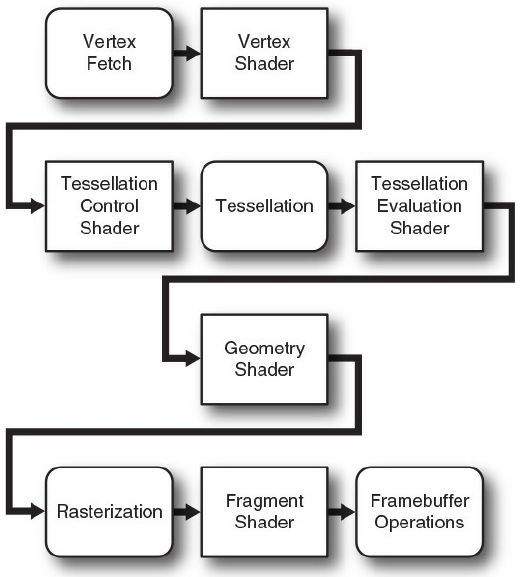
\includegraphics[width=0.75\textwidth]{graphicsPipeline}
	\caption{Упрощенная структура графического конвейера}%
    \label{fig:graphicsPipeline}
\end{figure}
На рисунке~\ref{fig:graphicsPipeline} блоки со скругленными краями представляют
собой фиксированные части, которые обычно реализованы как часть драйвера,
прошивки или другого системного ПО. Блоки с прямоугольными краями являются
программируемыми, это означает, что они могут выполнять шейдеры, предоставляемые
разработчиками ПО.

\section{Моделирование и визуализация огня}

Стохастические методы моделирования огня, такие как поля турбулентности и шумов
очень эффективны при создании реалистичного огня в 2D графике, но являются
крайне неэффективными по количеству операций для использования в 3D анимациях в
реальном времени, независимо от выбранной техники визуализации. Напротив,
эффективно релизованная объемная модель рендеринга, использующая воксели,
помогает достичь приемлемую для интерактивных приложений частоту кадров. Однако,
при использовании данной модели сложно добиться реалистичных результатов,
поскольку поверхность огня не имеет четких границ. Наиболее быстрым методом
является объемное моделирование с использованием полигонов для визуализации;
отрисовка полигонов происходит крайне быстро, однако полигоны не лучшее средство
для визуализации языков пламени, вихрящегося дыма и частиц сажи, и поэтому
обычно полигоны пораждают довольно грубые и низкокачественные результаты. Где-то
между ними находится моделирование с помощью систем частиц, данный метод может
работать с желаемой скоростью, в зависимости от выбранного масштаба, который
выбирается из расчета необходимого уровня детализации и выбранных техник
анимации и визуализации.
